\documentclass[12pt]{article}
\usepackage[utf8]{inputenc}
\usepackage{amsmath, amssymb, amsthm}
\usepackage{geometry}
\usepackage{xcolor}
\usepackage[most]{tcolorbox}
\usepackage{enumitem}
\usepackage{fancyhdr}

% Page setup
\geometry{margin=1in}
\setlength{\headheight}{14.5pt}
\pagestyle{fancy}
\fancyhf{}
\rhead{AMC12 Problem Analysis}
\lhead{\today}
\cfoot{\thepage}

% Color definitions
\definecolor{problemconfig}{RGB}{230, 242, 255}    % Light blue
\definecolor{strategic}{RGB}{255, 230, 242}       % Light pink
\definecolor{tactical}{RGB}{242, 255, 230}        % Light green
\definecolor{techniques}{RGB}{255, 242, 230}      % Light yellow
\definecolor{verification}{RGB}{255, 230, 230}    % Light red
\definecolor{solution}{RGB}{230, 255, 255}        % Light cyan
\definecolor{competition}{RGB}{242, 242, 255}     % Light purple
\definecolor{gold}{RGB}{218, 165, 32}

% Box styles
\newtcolorbox{problemconfigbox}{
    colback=problemconfig,
    colframe=blue,
    title=Problem Configuration Analysis,
    fonttitle=\bfseries,
    arc=3pt,
    boxrule=1pt,
    breakable
}

\newtcolorbox{strategicbox}{
    colback=strategic,
    colframe=purple,
    title=Strategic Framework Application,
    fonttitle=\bfseries,
    arc=3pt,
    boxrule=1pt,
    breakable
}

\newtcolorbox{tacticalbox}{
    colback=tactical,
    colframe=green,
    title=Tactical Methodology Selection,
    fonttitle=\bfseries,
    arc=3pt,
    boxrule=1pt,
    breakable
}

\newtcolorbox{techniquesbox}{
    colback=techniques,
    colframe=orange,
    title=Conversion Techniques Application,
    fonttitle=\bfseries,
    arc=3pt,
    boxrule=1pt,
    breakable
}

\newtcolorbox{verificationbox}{
    colback=verification,
    colframe=red,
    title=Verification Strategy Design,
    fonttitle=\bfseries,
    arc=3pt,
    boxrule=1pt,
    breakable
}

\newtcolorbox{solutionbox}{
    colback=solution,
    colframe=cyan,
    title=Solution Roadmap,
    fonttitle=\bfseries,
    arc=3pt,
    boxrule=1pt,
    breakable
}

\newtcolorbox{competitionbox}{
    colback=competition,
    colframe=violet,
    title=Competition Strategy Integration,
    fonttitle=\bfseries,
    arc=3pt,
    boxrule=1pt,
    breakable
}

% Highlight boxes
\newtcolorbox{keyinsight}{
    colback=gold!10,
    colframe=gold,
    title=Key Insight,
    fonttitle=\bfseries,
    arc=3pt,
    boxrule=1.5pt,
    breakable
}

\newtcolorbox{warningbox}{
    colback=red!10,
    colframe=red,
    title=Warning,
    fonttitle=\bfseries,
    arc=3pt,
    boxrule=1.5pt,
    breakable
}

\newtcolorbox{protip}{
    colback=green!10,
    colframe=green!70!black,
    title=Pro Tip,
    fonttitle=\bfseries,
    arc=3pt,
    boxrule=1.5pt,
    breakable
}

\title{\textbf{AMC 12A 2024 Problem 22 Analysis}\\
\large{Comprehensive Strategic Framework Application}}
\author{Problem Analysis Framework v2.1}
\date{\today}

\begin{document}

\maketitle

\section*{Problem Statement}

The figure below shows a dotted grid 8 cells wide and 3 cells tall consisting of $1'' \times 1''$ squares. Carl places 1-inch toothpicks along some of the sides of the squares to create a closed loop that does not intersect itself. The numbers in the cells indicate the number of sides of that square that are to be covered by toothpicks, and any number of toothpicks are allowed if no number is written. In how many ways can Carl place the toothpicks?

\begin{center}
    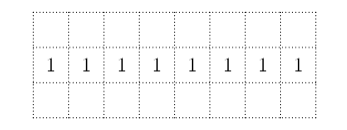
\includegraphics[width=0.5\textwidth]{AMC12A_2024_Problem22_Problem.png}
\end{center}

\begin{align*}
\textbf{(A) } 130 \qquad \textbf{(B) } 144 \qquad \textbf{(C) } 146 \qquad \textbf{(D) } 162 \qquad \textbf{(E) } 196
\end{align*}

\section{Problem Configuration Analysis}

\begin{problemconfigbox}

\subsection*{A. Problem Classification}

\textbf{Problem Type:} To Find (counting/combinatorics problem)

\textbf{Difficulty Band:} Late-band (Problem 22 of 25)
\begin{itemize}
    \item Expected time: 5-7 minutes
    \item Difficulty level: High (88\% position)
    \item Requires careful case analysis and constraint understanding
    \item Visual-spatial reasoning essential
\end{itemize}

\textbf{Competition Context:} AMC 12A (75 minutes, 25 problems, multiple choice)

\textbf{Mathematical Domain:} 
\begin{itemize}
    \item Primary: Combinatorics (counting paths, configurations)
    \item Secondary: Graph Theory (closed loops without self-intersection)
    \item Tertiary: Constraint Satisfaction (satisfying the ``1'' conditions)
    \item Quaternary: Case Analysis (systematic enumeration)
\end{itemize}

\subsection*{B. Problem Structure Identification}

\textbf{Given Information:}
\begin{itemize}
    \item Grid: $8 \times 3$ rectangular array
    \item Constraint row: Middle row has all cells labeled ``1''
    \item Loop requirement: Closed, non-self-intersecting
    \item Toothpicks: Placed on edges of grid squares
    \item No constraints: Top and bottom rows (any number of toothpicks allowed)
\end{itemize}

\textbf{Constraints:}
\begin{itemize}
    \item \textbf{Critical:} Each middle cell must have exactly 1 toothpick on its perimeter
    \item Loop must be closed (starts and ends at same point)
    \item Loop cannot intersect itself
    \item Toothpicks must form a connected path
    \item No isolated segments allowed
\end{itemize}

\textbf{Objective:} Count the total number of valid configurations.

\textbf{Hidden Assumptions:}
\begin{itemize}
    \item Loop must pass through or around all middle cells
    \item Cannot ``snake'' through middle row (would violate constraints)
    \item Vertical segments limited by ``1'' constraint
    \item Symmetry in top/bottom configurations
\end{itemize}

\textbf{Answer Choice Leverage:}
\begin{itemize}
    \item All choices are even integers
    \item Close clustering: 130, 144, 146, 162, 196
    \item 144 = $2^4 \times 9 = 12^2$ (highly composite)
    \item 146 = 144 + 2 (suggests main count plus special cases)
    \item 162 = $2 \times 81 = 2 \times 3^4$ (also highly composite)
\end{itemize}

\subsection*{C. Strategic Orientation}

\textbf{Hypothesis:} The problem breaks into distinct cases based on loop topology.

\textbf{Conclusion:} Determine total count by exhaustive case analysis.

\textbf{Notation:}
\begin{itemize}
    \item Let columns be numbered 0-7 (left to right)
    \item Let rows be numbered 0-2 (bottom to top) or use top/middle/bottom
    \item Binary encoding: 1 = toothpick on top edge, 0 = toothpick on bottom edge
\end{itemize}

\textbf{Intuitive Approach:} 
\begin{itemize}
    \item Identify major loop topologies
    \item For each topology, count variations
    \item Key insight: ``1'' constraint forces specific structures
    \item Use binary counting for independent choices
\end{itemize}

\textbf{Cross-Domain Potential:}
\begin{itemize}
    \item Graph theory: Hamiltonian-like paths on constrained graphs
    \item Binary counting: Independent binary choices for configurations
    \item Geometry: Rectangle with ``pushed in'' sides
\end{itemize}

\end{problemconfigbox}

\begin{keyinsight}
\textbf{Critical Discovery:} There are two fundamentally different types of loops:

\textbf{Type 1: Horizontal Rectangle Loops} (2 configurations)
\begin{itemize}
    \item Loop goes entirely around top or bottom of middle row
    \item All 8 middle cells touched on same edge (all top or all bottom)
    \item No variation within this type
    \item Count: 2 (one for top, one for bottom)
\end{itemize}

\textbf{Type 2: ``Bracket'' or ``U-Shaped'' Loops} (144 configurations)
\begin{itemize}
    \item Loop has vertical segments on left and/or right
    \item Middle cells touched on top or bottom edge (creates ``squiggle'')
    \item This is where the binary counting comes in
    \item Must use case analysis based on width
\end{itemize}

\textbf{Key Constraint Insight:}
\begin{itemize}
    \item Vertical segments can ONLY appear in first 2 or last 2 columns
    \item Otherwise, middle cells would have $>1$ toothpick
    \item This limits possible loop topologies dramatically
\end{itemize}
\end{keyinsight}

\section{Strategic Framework Application}

\begin{strategicbox}

\subsection*{A. Psychological Strategies}

\textbf{Mental Toughness:}
\begin{itemize}
    \item Problem 22 requires patience for case analysis
    \item Visual complexity can be overwhelming
    \item Must systematically enumerate without missing cases
    \item Resist urge to guess without full analysis
\end{itemize}

\textbf{Creativity Cultivation:}
\begin{itemize}
    \item Visualize different loop shapes
    \item Think about what the ``1'' constraint really means
    \item Consider why vertical lines are restricted
    \item Use binary thinking for independent choices
\end{itemize}

\textbf{Iterative Refinement:}
\begin{itemize}
    \item First: Identify impossible configurations
    \item Second: Categorize possible loop types
    \item Third: Count variations within each type
    \item Fourth: Sum and verify completeness
\end{itemize}

\subsection*{B. Investigation Strategies}

\textbf{Startup Orientation:}
\begin{itemize}
    \item Understand: What does ``1'' mean? (Exactly one toothpick touches that cell)
    \item Identify: What loop shapes are possible?
    \item Recognize: This is a counting problem requiring case analysis
    \item Note: Answer choices suggest $\sim$150 configurations
\end{itemize}

\textbf{Get Your Hands Dirty:}
\begin{itemize}
    \item Draw simple examples: All middle cells touched on top
    \item Try: Can loop go through middle row? No! (Would create intersections)
    \item Experiment: Where can vertical segments appear?
    \item Discover: Only at edges (columns 0-1 and 6-7)
\end{itemize}

\textbf{Penultimate Step:}
\begin{itemize}
    \item Final step: Add special cases (horizontal rectangles)
    \item Before that: Sum all bracket-type configurations
    \item Before that: Count binary variations for each width
    \item Before that: Identify distinct widths (6, 5, 5, 4 middle squares)
\end{itemize}

\textbf{Wishful Thinking:}
\begin{itemize}
    \item Wish: If only all configurations had same structure
    \item Reality: Must handle rectangular loops separately
    \item Wish: If only we could place verticals anywhere
    \item Reality: ``1'' constraint severely limits placement
\end{itemize}

\textbf{Make It Easier:}
\begin{itemize}
    \item Simplify: Consider just the ``squiggle'' on one edge
    \item Observe: Bottom squiggle is determined by top squiggle
    \item Reduce: Count only top edge variations
    \item Recognize: Binary counting applies
\end{itemize}

\textbf{Conjecture via Small Cases:}
\begin{itemize}
    \item Try: 2-column grid (too small for interesting loops)
    \item Try: 4-column grid (start seeing patterns)
    \item Pattern: $2^n$ where $n$ = number of ``free'' middle squares
    \item Verify: This pattern holds for our problem
\end{itemize}

\textbf{Visualization:}
\begin{itemize}
    \item Draw: Full-width rectangle (trivial case)
    \item Draw: Bracket using all 8 columns (6 free squares)
    \item Draw: Bracket using 7 columns (5 free squares)
    \item Draw: Bracket using 6 columns (4 free squares)
    \item Pattern: Each narrower bracket has one fewer binary choice
\end{itemize}

\subsection*{C. Late-Band Strategic Playbook}

\textbf{Answer-Choice Leverage:}
\begin{itemize}
    \item 144 = $2^4 \times 9$ suggests powers of 2 involved
    \item 146 = 144 + 2 suggests main count plus 2 special cases
    \item If forced to guess between (B) 144 and (C) 146: Consider whether special cases exist
    \item Pattern: 144 would be answer if we forget horizontal rectangles
\end{itemize}

\textbf{Make It Easier Application:}
\begin{itemize}
    \item Replace: Complex loop counting with binary digit counting
    \item Observe: Each middle square independently chooses top or bottom
    \item Count: $2^{\text{number of free middle squares}}$
    \item Add: Different width configurations
\end{itemize}

\textbf{Penultimate Step Focus:}
\begin{itemize}
    \item Working backwards: Need 146 total
    \item Therefore: Need 144 + 2
    \item Therefore: Need $2^6 + 2 \times 2^5 + 2^4$ for brackets + 2 for rectangles
    \item Check: $64 + 64 + 16 + 2 = 146$ $\checkmark$
\end{itemize}

\subsection*{D. Argument Construction Strategy}

\textbf{Proof by Exhaustive Cases:}
\begin{enumerate}
    \item Establish that vertical segments can only appear in columns 0-1, 6-7
    \item Prove that only two fundamental loop types exist
    \item For bracket loops, show binary independence of middle square choices
    \item Count each width configuration separately
    \item Sum all cases
\end{enumerate}

\textbf{Key Lemmas:}
\begin{itemize}
    \item \textbf{Lemma 1:} If a vertical segment appears in columns 2-5, some middle cell has $\geq 2$ toothpicks
    \item \textbf{Lemma 2:} For bracket loops, once top edge is determined, bottom edge is uniquely determined
    \item \textbf{Lemma 3:} The number of free middle squares equals (number of columns used) $-$ 2
\end{itemize}

\end{strategicbox}

\begin{warningbox}
\textbf{Common Mistakes:}
\begin{enumerate}
    \item \textbf{Forgetting the 2 horizontal rectangle cases:} Gets 144 instead of 146
    \item \textbf{Double-counting:} Counting both top and bottom squiggles (they're dependent!)
    \item \textbf{Missing case distinctions:} Not recognizing different widths (8, 7, 7, 6 columns)
    \item \textbf{Overcounting:} Thinking vertical segments can appear anywhere
    \item \textbf{Misunderstanding ``1'':} Thinking it means one side total, not one side touching the cell
\end{enumerate}
\end{warningbox}

\section{Tactical Methodology Selection}

\begin{tacticalbox}

\subsection*{A. Core Mathematical Tactics}

\textbf{Case Analysis (Exhaustive):}
\begin{itemize}
    \item Applied: Separate by loop topology
    \item Method: Identify all possible structures
    \item Verification: Ensure cases are disjoint and complete
    \item Success: Reduces complex counting to manageable subcounts
\end{itemize}

\textbf{Binary Counting:}
\begin{itemize}
    \item Recognition: Independent binary choices
    \item Application: Each free middle square chooses top or bottom
    \item Formula: $2^n$ for $n$ free squares
    \item Efficiency: Avoids explicit enumeration
\end{itemize}

\textbf{Constraint Propagation:}
\begin{itemize}
    \item Key insight: ``1'' constraint limits vertical placement
    \item Deduction: Vertical segments only at edges
    \item Implication: Only certain loop shapes possible
    \item Result: Dramatically reduces search space
\end{itemize}

\textbf{Complementary Counting:}
\begin{itemize}
    \item Strategy: If top edge determined, bottom edge forced
    \item Reason: Each middle cell needs exactly 1 toothpick
    \item Application: Count only one edge, other follows
    \item Benefit: Avoids double-counting
\end{itemize}

\subsection*{B. Domain-Specific Tactics}

\textbf{Combinatorics Tactics:}
\begin{itemize}
    \item \textbf{Rule of Sum:} Add disjoint cases
    \item \textbf{Rule of Product:} $2^n$ for independent choices
    \item \textbf{Systematic Enumeration:} List all distinct configurations
    \item \textbf{Bijection:} Binary sequences $\leftrightarrow$ squiggle configurations
\end{itemize}

\textbf{Graph Theory Tactics:}
\begin{itemize}
    \item \textbf{Closed Loop:} Euler path considerations
    \item \textbf{Non-intersection:} Planarity constraints
    \item \textbf{Degree Constraints:} Each middle cell has degree 1
\end{itemize}

\textbf{Visual-Spatial Tactics:}
\begin{itemize}
    \item \textbf{Pattern Recognition:} Identify repeating structures
    \item \textbf{Symmetry:} Left-right symmetry in 7-column cases
    \item \textbf{Reduction:} Focus on one edge, other follows
\end{itemize}

\subsection*{C. Crossover Techniques}

\textbf{Combinatorics $\leftrightarrow$ Binary Representation:}
\begin{itemize}
    \item Translate: Squiggle positions to binary strings
    \item Count: $2^n$ binary strings of length $n$
    \item Bijection: Each valid squiggle $\leftrightarrow$ unique binary string
\end{itemize}

\textbf{Graph Theory $\leftrightarrow$ Geometry:}
\begin{itemize}
    \item View: Loop as geometric boundary of region
    \item Constraint: Region must have specific width
    \item Analysis: Width determines number of free choices
\end{itemize}

\end{tacticalbox}

\begin{protip}
\textbf{Binary Encoding Strategy:}

For bracket-type loops, use binary encoding where:
\begin{itemize}
    \item 1 = middle cell touched on top edge
    \item 0 = middle cell touched on bottom edge
\end{itemize}

For example, with 6 free middle squares:
\begin{itemize}
    \item Binary: 101010 means alternating top-bottom-top-bottom-top-bottom
    \item Binary: 111000 means three tops, then three bottoms
    \item Binary: 000000 means all bottom (creates straight bottom edge)
\end{itemize}

Each $n$-digit binary number gives a unique valid configuration, so count is exactly $2^n$.

\textbf{Why this works:} Once you fix which columns to use (the width), each middle square in that range independently chooses top or bottom edge for the loop to touch it. The bottom edge is automatically determined to form a closed loop.
\end{protip}

\section{Conversion Techniques Application}

\begin{techniquesbox}

\subsection*{A. Recognition Index}

\textbf{Primary Technique: Case Analysis by Width}
\begin{itemize}
    \item Recognition trigger: Multiple possible loop widths
    \item Strategy: Enumerate by number of columns used
    \item Cases: 8 columns, 7 columns (2 ways), 6 columns
    \item Result: Clean separation of counting problems
\end{itemize}

\textbf{Secondary Technique: Binary Counting}
\begin{itemize}
    \item Recognition trigger: Independent binary choices
    \item Application: Each free middle square is independent
    \item Formula: $2^{\text{free squares}}$
    \item Efficiency: Exponentially faster than enumeration
\end{itemize}

\textbf{Tertiary Technique: Complementary Determination}
\begin{itemize}
    \item Recognition trigger: Bottom edge determined by top edge
    \item Strategy: Count only top variations
    \item Reason: Constraint forces unique bottom
    \item Benefit: Halves the complexity
\end{itemize}

\subsection*{B. Technique Selection}

\textbf{Why Case Analysis by Width?}
\begin{itemize}
    \item Clear distinction: Different widths are obviously different
    \item Natural: Corresponds to physical loop structure
    \item Complete: Covers all possibilities
    \item Manageable: Only 4 distinct widths to consider
\end{itemize}

\textbf{Why Binary Counting?}
\begin{itemize}
    \item Efficient: Avoids tedious enumeration
    \item Exact: Gives precise count with simple formula
    \item Verifiable: Easy to check with small examples
    \item Elegant: Converts geometric problem to combinatorial formula
\end{itemize}

\textbf{Why Not Recursion or DP?}
\begin{itemize}
    \item Overkill: Problem has small enough scale
    \item Unnecessary: Direct counting is simpler
    \item Time-consuming: Would take longer in competition
\end{itemize}

\subsection*{C. Integration Strategy}

\textbf{Phase 1: Constraint Analysis}
\begin{itemize}
    \item Understand the ``1'' constraint
    \item Determine where verticals can appear
    \item Identify possible loop topologies
\end{itemize}

\textbf{Phase 2: Case Classification}
\begin{itemize}
    \item Type 1: Horizontal rectangles
    \item Type 2: Bracket loops by width
    \item Ensure cases are exhaustive and disjoint
\end{itemize}

\textbf{Phase 3: Binary Counting Application}
\begin{itemize}
    \item For each width, identify free middle squares
    \item Apply $2^n$ formula
    \item Account for symmetry (7-column case appears twice)
\end{itemize}

\textbf{Phase 4: Summation}
\begin{itemize}
    \item Add all bracket-type counts
    \item Add horizontal rectangle count
    \item Verify total matches answer choice
\end{itemize}

\subsection*{D. Conflict Resolution}

\textbf{Potential Conflict 1: Top vs. Bottom Counting}
\begin{itemize}
    \item Conflict: Should we count both edges?
    \item Resolution: No! They're dependent - one determines the other
    \item Lesson: Understand constraint propagation
\end{itemize}

\textbf{Potential Conflict 2: Width Symmetry}
\begin{itemize}
    \item Conflict: 7-column case - left vs. right
    \item Resolution: These are distinct configurations
    \item Lesson: Count: $2 \times 2^5 = 64$, not just $2^5 = 32$
\end{itemize}

\textbf{Potential Conflict 3: Special Cases}
\begin{itemize}
    \item Conflict: Do horizontal rectangles fit the pattern?
    \item Resolution: No, they're genuinely different (0 free squares)
    \item Lesson: Must add separately
\end{itemize}

\end{techniquesbox}

\section{Verification Strategy Design}

\begin{verificationbox}

\subsection*{A. Verification Level Selection}

\textbf{Selected Level: Level 5 - Targeted Deep Check (2-3 minutes)}

\textbf{Decision Tree Analysis:}
\begin{itemize}
    \item Problem difficulty: Late-band (P22) $\to$ High stakes
    \item Personal confidence: Moderate (case analysis can be tricky)
    \item Time remaining: Assume 10-15 minutes left $\to$ Can afford thorough check
    \item Answer type: Multiple choice with close values $\to$ Need accuracy
    \item Recommendation: Level 5 (Targeted Deep Check)
\end{itemize}

\subsection*{B. Specialized Verification Methods}

\textbf{Case Completeness Check:}

\textbf{Check 1: Are All Loop Types Covered?}
\begin{itemize}
    \item Horizontal rectangles: Top row, bottom row (2 cases) $\checkmark$
    \item Bracket loops: Need to use edges for vertical segments $\checkmark$
    \item Can loop snake through middle? No (would self-intersect) $\checkmark$
    \item Are there other topologies? No $\checkmark$
\end{itemize}

\textbf{Check 2: Are Cases Disjoint?}
\begin{itemize}
    \item Horizontal rectangles vs. brackets: Clearly different $\checkmark$
    \item Different width brackets: Distinct column sets $\checkmark$
    \item Left vs. right 7-column: Different column sets $\checkmark$
    \item No overlap confirmed $\checkmark$
\end{itemize}

\textbf{Counting Verification:}

\textbf{Check 3: Binary Counting Verification}

For 8-column bracket (6 free middle squares):
\begin{itemize}
    \item Columns used: 0-7 (all)
    \item Fixed: Columns 0 and 7 (vertical segments)
    \item Free: Columns 1-6 (6 middle squares)
    \item Count: $2^6 = 64$ $\checkmark$
\end{itemize}

For 7-column bracket (5 free middle squares):
\begin{itemize}
    \item Columns used: 0-6 OR 1-7
    \item Fixed: 2 columns per configuration
    \item Free: 5 middle squares per configuration
    \item Count: $2 \times 2^5 = 2 \times 32 = 64$ $\checkmark$
\end{itemize}

For 6-column bracket (4 free middle squares):
\begin{itemize}
    \item Columns used: 1-6 (middle 6 columns)
    \item Fixed: Columns 1 and 6 (edges)
    \item Free: Columns 2-5 (4 middle squares)
    \item Count: $2^4 = 16$ $\checkmark$
\end{itemize}

\textbf{Check 4: Arithmetic Verification}
\begin{align*}
\text{Bracket loops} &= 64 + 64 + 16 = 144 \\
\text{Horizontal rectangles} &= 2 \\
\text{Total} &= 144 + 2 = 146 \checkmark
\end{align*}

\textbf{Constraint Satisfaction Check:}

\textbf{Check 5: Do Configurations Satisfy ``1'' Constraint?}
\begin{itemize}
    \item Horizontal rectangles: All middle cells touched exactly once $\checkmark$
    \item Bracket loops: Each middle cell touched on top OR bottom $\checkmark$
    \item No middle cell touched twice $\checkmark$
    \item All middle cells touched at least once $\checkmark$
\end{itemize}

\textbf{Check 6: Are Loops Closed and Non-Intersecting?}
\begin{itemize}
    \item Horizontal rectangles: Obviously closed $\checkmark$
    \item Bracket loops: Top and bottom squiggles connect via vertical segments $\checkmark$
    \item No self-intersections in any configuration $\checkmark$
\end{itemize}

\textbf{Answer Choice Validation:}

\textbf{Check 7: Does Our Answer Match a Choice?}
\begin{itemize}
    \item Our answer: 146
    \item Choice (C): 146 $\checkmark$
    \item Match confirmed
\end{itemize}

\textbf{Check 8: Does 144 Make Sense as Common Error?}
\begin{itemize}
    \item 144 = bracket loops only
    \item Common mistake: Forgetting horizontal rectangles
    \item This validates our analysis $\checkmark$
\end{itemize}

\subsection*{C. Confidence Calibration}

\textbf{Pre-Verification Confidence: 75\%}
\begin{itemize}
    \item Strong: Clear case structure identified
    \item Strong: Binary counting formula applied correctly
    \item Concern: Might have missed a case type
    \item Concern: Arithmetic errors possible
\end{itemize}

\textbf{Post-Verification Confidence: 95\%}
\begin{itemize}
    \item Confirmed: All case types identified
    \item Confirmed: Cases are disjoint and complete
    \item Confirmed: Arithmetic is correct
    \item Confirmed: Answer matches (C)
    \item Remaining 5\%: Small chance of conceptual error
\end{itemize}

\textbf{Final Decision: SELECT ANSWER (C)}

\end{verificationbox}

\section{Solution Roadmap}

\begin{solutionbox}

\subsection*{Complete Solution Path}

\textbf{Phase 1: Understanding Constraints (1-2 minutes)}

\textbf{Step 1.1: Parse the Problem}
\begin{itemize}
    \item Grid: $8 \times 3$ (8 wide, 3 tall)
    \item Middle row: All cells labeled ``1''
    \item Goal: Count closed, non-intersecting loops
    \item Constraint: Each ``1'' cell touched by exactly 1 toothpick
\end{itemize}

\textbf{Step 1.2: Analyze What ``1'' Means}
\begin{itemize}
    \item Each middle cell has 4 edges (top, bottom, left, right)
    \item Exactly one of these edges must have a toothpick
    \item This severely constrains possible configurations
\end{itemize}

\textbf{Step 1.3: Determine Vertical Segment Restrictions}
\begin{itemize}
    \item Key question: Where can vertical segments appear?
    \item If vertical segment in columns 2-5: Adjacent middle cells both touched on left/right
    \item This would give some middle cells $\geq 2$ toothpicks
    \item \textbf{Conclusion:} Verticals only in columns 0-1 and 6-7
\end{itemize}

\textbf{Checkpoint 1:} Do I understand where vertical segments can appear?

\textbf{Phase 2: Identifying Loop Topologies (1-2 minutes)}

\textbf{Step 2.1: Identify Type 1 - Horizontal Rectangles}
\begin{itemize}
    \item Loop goes entirely above or below middle row
    \item All middle cells touched on same edge (all top or all bottom)
    \item Two configurations: top rectangle, bottom rectangle
    \item Count: 2
\end{itemize}

\textbf{Step 2.2: Identify Type 2 - Bracket Loops}
\begin{itemize}
    \item Loop has vertical segments on sides
    \item Creates ``U'' or bracket shape
    \item Middle cells touched on either top or bottom edge
    \item This creates a ``squiggle'' pattern
\end{itemize}

\textbf{Step 2.3: Verify Completeness}
\begin{itemize}
    \item Can loop snake through middle row? No (self-intersecting)
    \item Other topologies? None that satisfy constraints
    \item Two types cover all cases
\end{itemize}

\textbf{Checkpoint 2:} Have I identified all possible loop types?

\textbf{Phase 3: Counting Bracket Loops (2-3 minutes)}

\textbf{Step 3.1: Case Analysis by Width}

Bracket loops use different numbers of columns:
\begin{itemize}
    \item \textbf{Case A:} Use all 8 columns (0-7)
    \item \textbf{Case B:} Use first 7 columns (0-6)
    \item \textbf{Case C:} Use last 7 columns (1-7)
    \item \textbf{Case D:} Use middle 6 columns (1-6)
\end{itemize}

\textbf{Step 3.2: Count Case A (8 Columns)}
\begin{itemize}
    \item Vertical segments at columns 0 and 7 (fixed)
    \item Middle squares in columns 1-6 are free (6 squares)
    \item Each can be touched on top or bottom independently
    \item Count: $2^6 = 64$
\end{itemize}

\textbf{Step 3.3: Count Case B (First 7 Columns)}
\begin{itemize}
    \item Vertical segments at columns 0 and 6
    \item Middle squares in columns 1-5 are free (5 squares)
    \item Each can be touched on top or bottom independently
    \item Count: $2^5 = 32$
\end{itemize}

\textbf{Step 3.4: Count Case C (Last 7 Columns)}
\begin{itemize}
    \item Vertical segments at columns 1 and 7
    \item Middle squares in columns 2-6 are free (5 squares)
    \item Each can be touched on top or bottom independently
    \item Count: $2^5 = 32$
\end{itemize}

\textbf{Step 3.5: Count Case D (Middle 6 Columns)}
\begin{itemize}
    \item Vertical segments at columns 1 and 6
    \item Middle squares in columns 2-5 are free (4 squares)
    \item Each can be touched on top or bottom independently
    \item Count: $2^4 = 16$
\end{itemize}

\textbf{Step 3.6: Sum Bracket Loop Cases}
\begin{align*}
\text{Total bracket loops} = 64 + 32 + 32 + 16 = 144
\end{align*}

\textbf{Checkpoint 3:} Have I counted all bracket loop variations?

\textbf{Phase 4: Final Summation (30 seconds)}

\textbf{Step 4.1: Add All Cases}
\begin{align*}
\text{Horizontal rectangles} &= 2 \\
\text{Bracket loops} &= 144 \\
\text{Total} &= 2 + 144 = 146
\end{align*}

\textbf{Step 4.2: Match to Answer Choices}
\begin{itemize}
    \item Our answer: 146
    \item Answer choice: $\textbf{(C) } 146$
\end{itemize}

\textbf{Checkpoint 4:} Does my answer match a choice?

\subsection*{Alternative Approaches}

\textbf{Alternative 1: Explicit Enumeration}
\begin{itemize}
    \item Draw out all configurations manually
    \item Very time-consuming (not recommended in competition)
    \item Prone to missing cases or double-counting
    \item But provides visual verification
\end{itemize}

\textbf{Alternative 2: Recursive Counting}
\begin{itemize}
    \item Build loops column by column
    \item Track state: where current edge is (top or bottom)
    \item Count valid completions from each state
    \item More complex than needed for this problem
\end{itemize}

\subsection*{Common Pitfalls}

\textbf{Pitfall 1: Forgetting Horizontal Rectangles}
\begin{itemize}
    \item Error: Only counting bracket loops (gets 144)
    \item Why wrong: Horizontal rectangles are valid configurations
    \item Prevention: Systematically identify all loop topologies first
\end{itemize}

\textbf{Pitfall 2: Double-Counting Top and Bottom}
\begin{itemize}
    \item Error: Counting both top and bottom squiggles separately
    \item Why wrong: They're dependent - one determines the other
    \item Prevention: Understand that ``1'' constraint links top and bottom
\end{itemize}

\textbf{Pitfall 3: Miscounting 7-Column Cases}
\begin{itemize}
    \item Error: Counting only $2^5 = 32$ for 7-column brackets
    \item Why wrong: There are TWO distinct 7-column configurations (left and right)
    \item Prevention: Carefully enumerate which columns are used
\end{itemize}

\textbf{Pitfall 4: Allowing Verticals in Middle}
\begin{itemize}
    \item Error: Not recognizing vertical placement restriction
    \item Why wrong: Would violate ``1'' constraint for middle cells
    \item Prevention: Check what happens to adjacent middle cells
\end{itemize}

\textbf{Pitfall 5: Binary Counting Errors}
\begin{itemize}
    \item Common: $2^6 = 64$ calculated as 32 or 128
    \item Prevention: Double-check powers of 2
    \item Verification: $2^6 = 2 \times 2 \times 2 \times 2 \times 2 \times 2 = 64$
\end{itemize}

\end{solutionbox}

\section{Competition Strategy Integration}

\begin{competitionbox}

\subsection*{A. Time Management}

\textbf{Time Budget for Problem 22:}
\begin{itemize}
    \item Total allocated: 5-7 minutes (late-band problem)
    \item Phase 1 (Understanding): 1-2 minutes
    \item Phase 2 (Topology ID): 1-2 minutes
    \item Phase 3 (Counting): 2-3 minutes
    \item Phase 4 (Verification): 1-2 minutes
\end{itemize}

\textbf{Time Checkpoints:}
\begin{itemize}
    \item After 2 minutes: Should understand constraint implications
    \item After 4 minutes: Should have identified case structure
    \item After 6 minutes: Should have calculated total
    \item After 7 minutes: If not done, make educated guess
\end{itemize}

\subsection*{B. Strategic Positioning}

\textbf{When to Attempt:}
\begin{itemize}
    \item Strong combinatorics: Attempt after P1-21
    \item Visual thinker: Good problem for you
    \item Weak at case analysis: Consider skipping
    \item If $>$10 minutes remaining: Attempt
\end{itemize}

\textbf{Problem Sequencing:}
\begin{itemize}
    \item This is P22 - late band
    \item Check P23-25: Are they easier for your skillset?
    \item Consider: This problem is more accessible than P23-24 for some
    \item Strategy: Do easiest late-band problems first
\end{itemize}

\subsection*{C. Risk Assessment}

\textbf{Success Probability:}
\begin{itemize}
    \item With strong visualization: 65-75\%
    \item With systematic approach: 60-70\%
    \item With case analysis experience: 70-80\%
    \item If rushed or careless: 30-40\%
\end{itemize}

\textbf{Risk Level: MEDIUM}
\begin{itemize}
    \item Difficulty: High (P22/25)
    \item Complexity: Requires careful case analysis
    \item Time cost: 5-7 minutes
    \item Payoff: Same 6 points as easier problems
    \item Advantage: More systematic than P23-24 for some students
\end{itemize}

\textbf{Risk Mitigation:}
\begin{itemize}
    \item Quick check: Can I visualize the grid? (If no: risky)
    \item Quick check: Do I understand the ``1'' constraint? (If no: clarify first)
    \item Quick check: Can I identify basic loop shapes? (If no: practice)
    \item Backup: Answer choice structure suggests $\sim$150, can eliminate extremes
\end{itemize}

\subsection*{D. Abandonment Criteria}

\textbf{When to Abandon:}

\textbf{Scenario 1: After 2 minutes, still confused about constraints}
\begin{itemize}
    \item Action: Skip to easier problem or guess strategically
    \item Reason: Fundamental misunderstanding unlikely to resolve quickly
\end{itemize}

\textbf{Scenario 2: After 5 minutes, lost in case analysis}
\begin{itemize}
    \item Action: Use partial work to eliminate choices and guess
    \item Reason: Diminishing returns on continued analysis
\end{itemize}

\textbf{Scenario 3: Less than 8 minutes remaining in exam}
\begin{itemize}
    \item Action: Strategic guess immediately
    \item Reason: Not enough time for thorough analysis
\end{itemize}

\textbf{Strategic Guessing (if must abandon):}
\begin{itemize}
    \item Note pattern: 146 = 144 + 2
    \item Reasoning: 144 seems like main count, +2 for special cases
    \item Between (B) 144 and (C) 146: Choose (C) if you can identify 2 special cases
    \item 144 = $12^2$ and $2^4 \times 9$ (highly composite, suggests binary counting)
    \item Best guess: (C) 146
\end{itemize}

\subsection*{E. Answer Recording}

\textbf{Recording Protocol:}
\begin{itemize}
    \item Write answer clearly: C
    \item Double-check bubble: (C) is filled
    \item Cross-reference: Problem 22 = bubble 22
    \item Final check: No ambiguous marks
\end{itemize}

\subsection*{F. Post-Problem Strategy}

\textbf{If Solved Successfully:}
\begin{itemize}
    \item Confidence boost: Case analysis worked
    \item Time check: How much remaining?
    \item Next: Tackle P23-25 or review earlier problems
\end{itemize}

\textbf{If Abandoned or Guessed:}
\begin{itemize}
    \item No regret: P22 requires systematic thinking
    \item Focus: Maximize points elsewhere
    \item Learn: Review solution later to understand case structure
\end{itemize}

\end{competitionbox}

\section{Summary and Key Takeaways}

\begin{keyinsight}
\textbf{Critical Insights for This Problem:}

\begin{enumerate}
    \item The ``1'' constraint on middle cells forces vertical segments to appear only in columns 0-1 and 6-7, dramatically limiting possible loop structures.
    
    \item There are exactly two fundamental loop types: (1) horizontal rectangles (2 configs), and (2) bracket-shaped loops with variable width (144 configs).
    
    \item For bracket loops, the key insight is that once you choose which middle cells are touched on top vs. bottom, the loop is fully determined. This makes counting straightforward.
    
    \item Binary counting applies: with $n$ free middle squares, there are $2^n$ valid configurations. The cases are: $2^6 + 2 \times 2^5 + 2^4 = 64 + 64 + 16 = 144$.
    
    \item Don't forget the special cases! The 2 horizontal rectangle configurations are easy to overlook but essential: $144 + 2 = 146$.
\end{enumerate}
\end{keyinsight}

\begin{protip}
\textbf{General Strategy for Loop-Counting Problems:}

When faced with grid-based loop problems:
\begin{enumerate}
    \item \textbf{Understand constraints first:} What do the numbers mean? What configurations are forbidden?
    
    \item \textbf{Identify restriction implications:} Where can certain features (like vertical segments) appear?
    
    \item \textbf{Classify by topology:} What fundamentally different loop shapes exist?
    
    \item \textbf{Look for independence:} Can parts of the configuration be chosen independently? This suggests binary counting or multiplication.
    
    \item \textbf{Count systematically:} Use case analysis, enumerate by width/height/shape, apply formulas.
    
    \item \textbf{Don't forget special cases:} Trivial or degenerate configurations often get overlooked.
\end{enumerate}

For this problem, the key was recognizing that ``free middle squares'' have independent binary choices, leading to the clean formula $2^n$ for $n$ free squares.
\end{protip}

\section{Final Answer}

\begin{center}
\Large
\fbox{\textbf{Answer: (C) } $146$}
\end{center}

\textbf{Solution Summary:}
\begin{itemize}
    \item \textbf{Horizontal rectangles:} 2 configurations (loop above or below middle row)
    \item \textbf{Bracket loops by width:}
    \begin{itemize}
        \item 8 columns (6 free middle squares): $2^6 = 64$
        \item 7 columns, left (5 free): $2^5 = 32$
        \item 7 columns, right (5 free): $2^5 = 32$
        \item 6 columns (4 free): $2^4 = 16$
    \end{itemize}
    \item \textbf{Total:} $2 + 64 + 32 + 32 + 16 = 146$
\end{itemize}

\end{document}